\startfirstchapter{Introduction}

\section{Motivation}
The research of this Thesis is motivated by the recognized need for practical technologies that can cultivate a sustainable society. The two social problems that are addressed by this Thesis are water insecurity and antimicrobial resistance (AMR), which converge in membrane desalination research. The intention of this Thesis is to offer application programming interfaces (APIs) as computational tools that can facilitate the necessary development of these practical technologies and thereby ensure that water security and efficacious medical treatments are sustainable facets of our society.

\section{Water security}
Fresh water resources are diminishing \cite{Laghari2013MeltingUncertainty,Rasul2008GlobalRanges}, despite that water is one of the most abundant chemicals on Earth \cite{Shiklomanov1993WorldResources}. This is a consequence of global warming \cite{Hansen2006GlobalChange,IPCC2018Global1.5C} and climate change \cite{Thomas2004ExtinctionChange} that disrupt the water cycle, and pollution \cite{Pappas2017EnergySuperpower,Zhao2016DecouplingInvestment,Moller2010DistributionWatershed} and over-consumption \cite{Bongaarts2009HumanTransition,Meyer1992HumanChange} that contaminate and deplete water reserves, respectively. One of the many consequences of less available freshwater is that billions of people \cite{Unicef2017ThirstingClimate}, who disproportionately reside in developing nations, experience water insecurity each year\cite{Hoekstra2012GlobalAvailability}. This disparity in access to potable water is recognized as a top global challenge in the 6th UN Sustainable Development Goal \cite{Jones2018TheOutlook}. 

Desalination is a promising technology that may resolve water insecurities. Desalination enables municipalities to generate potable freshwater from diverse feed sources: especially the oceans \cite{2018DepartmentWater,Service2006DesalinationUp}, which are both within $100 km$ for $\approx \frac{1}{2}$ of the human population \cite{Amy2017Membrane-basedProspects} and are practically inexhaustible relative to the magnitude of human consumption. Desalination methods vary; however, membrane methods such as spiral-wound reverse osmosis (RO) are most common since they optimize the filtration surface area  per unit volume. A cross-sectional schema of RO is represented in Figure \ref{membrane_schema}. These membranes, when operational, selectively permit the diffusion of water across the membrane, while dissolved and suspended impurities are retained in the feed channel. The accumulation of ions, chemicals, and microorganisms in the feed channel during desalination gradually causes membrane fouling \cite{Goosen2004FoulingReview}, which hinders RO efficacy. The two primary types of fouling are biofouling \cite{Characklis1983BiofilmsFouling} -- microbial colonization of the polymeric filtration membrane \cite{Garcia-Trinanes2021InvestigatingDevice,Suwarno2014BiofoulingDevelopment} -- and scaling -- mineral precipitation and deposition upon the membrane surface \cite{Warsinger2015ScalingReview,Khan2013SourceSea,Tang2014FoulingPlant,Shmulevsky2017AnalysisMembranes}. 

\begin{figure}[b]
    \centering
    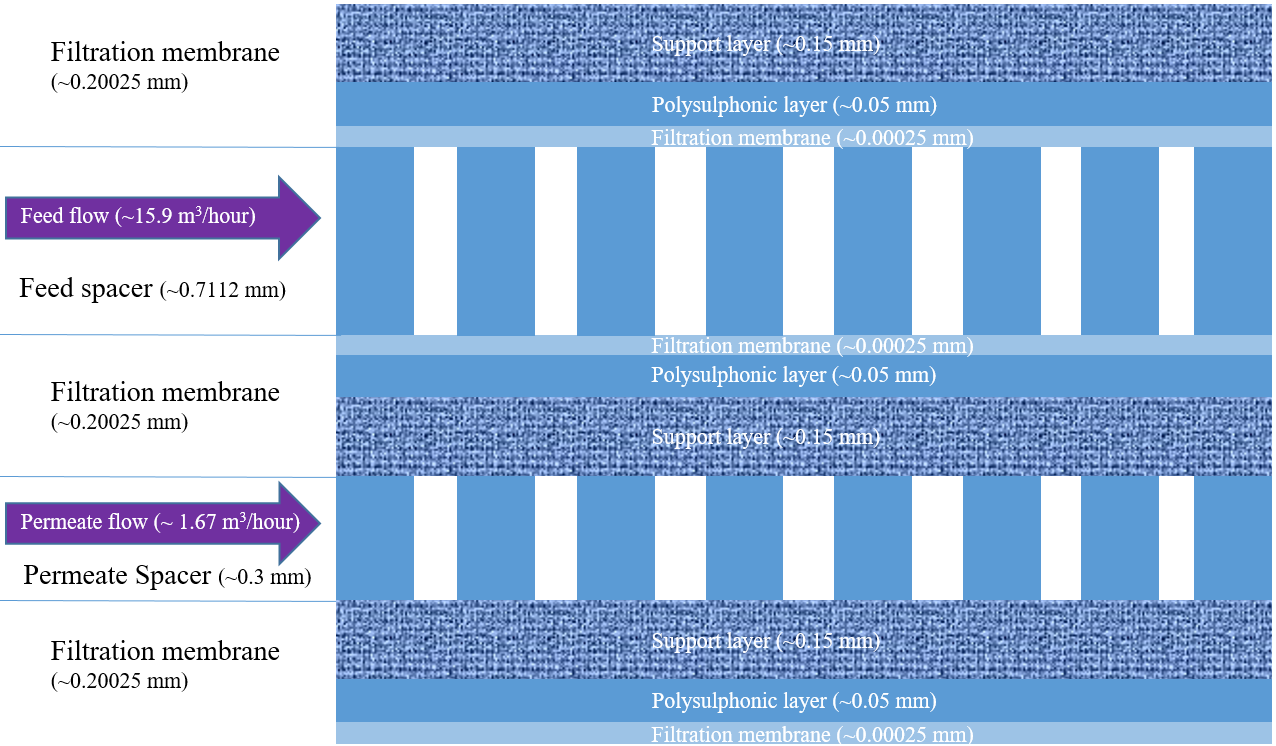
\includegraphics[width = \textwidth]{images/Introduction/membrane_schema_3.PNG}
    \caption{
        A cross-section of the RO polyamide filtration membrane \cite{Strubbe2018CalibrationFull-Scale}. 
    }
    \label{membrane_schema}
\end{figure}

\subsection{Scaling}
Scaling is a geochemical phenomena, which is depicted in Figure \ref{desalination_schema}, that can occlude and tear the filtration membrane. The geochemical equilibria that result in scaling are difficult to experimentally study; hence, computational software that predict scaling from the first principles of chemical equilibria. These software, however, are generally esoteric, expensive, and not API accessible, which limits their accessibility and their compatibility with large-scale simulations. We therefore developed ROSSpy (Reverse Osmosis Scaling Software in Python) as an intuitive and open-source API to provide the community with a unique resource to predict scaling from a parameterized RO system. ROSSpy  implements an original model that simplifies desalination into a one-dimensional reactive transport process, which is detailed with examples and use cases in Chapter \ref{ROSSpy_chapter}.

\begin{figure}[h]
    \centering
    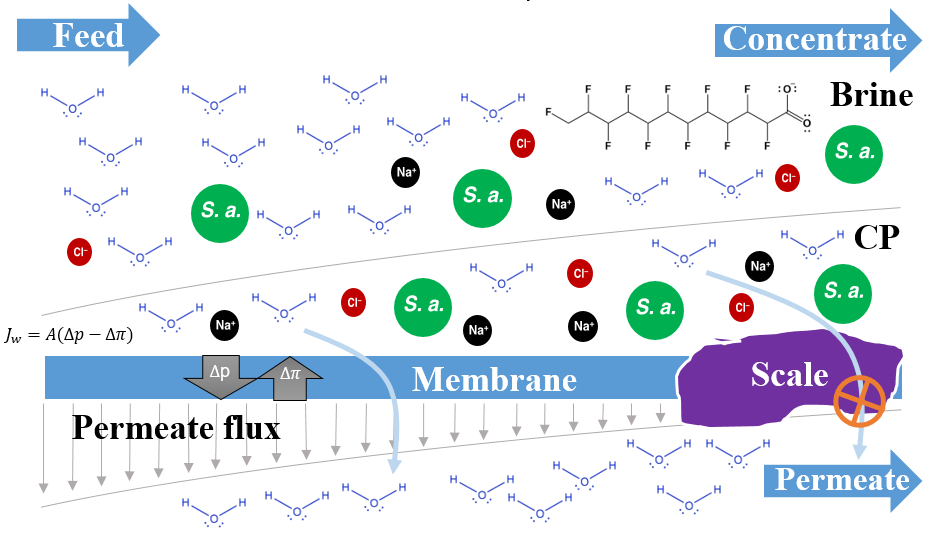
\includegraphics[width = \textwidth]{images/Introduction/desalination_schema_3.PNG}
    \caption{
        A cross-section perspective of RO desalination, which depicts the geochemical reactive transport through the module and the physical hindrance of scaling upon the membrane surface.  The flux through the membrane decreases over the module distance as a function of the pressure difference between the applied pressure of the feed and the osmotic pressure between the filtered (permeate) water and brine (concentrate) solution.  
    }
    \label{desalination_schema}
\end{figure}

\subsection{Biofouling}
Biofouling from microbial communities (biofilms) is another hindrance to RO desalination \cite{Flemming1997ReverseBiofouling,Ridgway1991BiofoulingMembranes,Ivnitsky2005CharacterizationTreatment,Herzberg2007BiofoulingPressure,Schneider2005DynamicsBiofouling,Flemming1997BiofoulingProcesses,Cantor1969BiologicalMembranes,Murphy2001MicrobiologicalMembranes,Chen2004CommunityApproach}. Biocidal treatments can limit biofouling \cite{Kim2009BiocideOverview}, however, these treatments have substantial collateral effects of chemically degrading the filtration membrane \cite{Da-Silva-Correa2022TheReview} and/or causing persistent ecotoxic effects in the environment \cite{Martins2018Review:Ecosystems,Thomas2001AntifoulingEffects}. The design of benign anti-biofoulants \cite{Buckley2017DesignProducts} is therefore essential to improve the efficacy and sustainability of RO desalination. Innovation here \cite{Winters1983ControlDesalination} can be accelerated by computational tools that allow experimentalists to predict the effect of different combinations of benign chemical agents and biofilm conditions. We therefore developed the WCMpy (Whole Cell Model in Python) suite of packages to foster the development of such computational tools, which is detailed in Chapter \ref{WCMpy_chapter}. 

\section{Antimicrobial resistance}
Infections from AMR are projected to exceed cancer in annual deaths, and globally cost $10^{13}~USD$ in lost economic production, by mid-21st century \cite{ONeill2014AntimicrobialNations}. The AMR crisis may be mitigated through the use of reactive oxygen species (ROSs), which non-selectively oxidize and kill pathogens while avoiding the mechanisms that result in AMR. ROSs can be wielded and controlled through photodynamic inactivation (PDI) systems that generate ROSs, primarily singlet oxygen ($\ce{^1O_2}$), on demand whenever light is shown upon the system. This photochemical process of PDI is catalyzed by a photosensitizer (PS) chemical, which is illustrated in Figure \ref{PDI_workflow}. The innumerable possible combinations of PSs and undesirable microbial targets are unlikely to be completely explored with experiments before mid-century, since resource limitations restrain experimentation; therefore, we developed PDIpy (Photodynamic Inactivation in Python) as a module to predict the efficacy for a range of possible PDI systems. This project is detailed in Chapter \ref{PDIpy_chapter}. 

\begin{figure}[h]
    \centering
    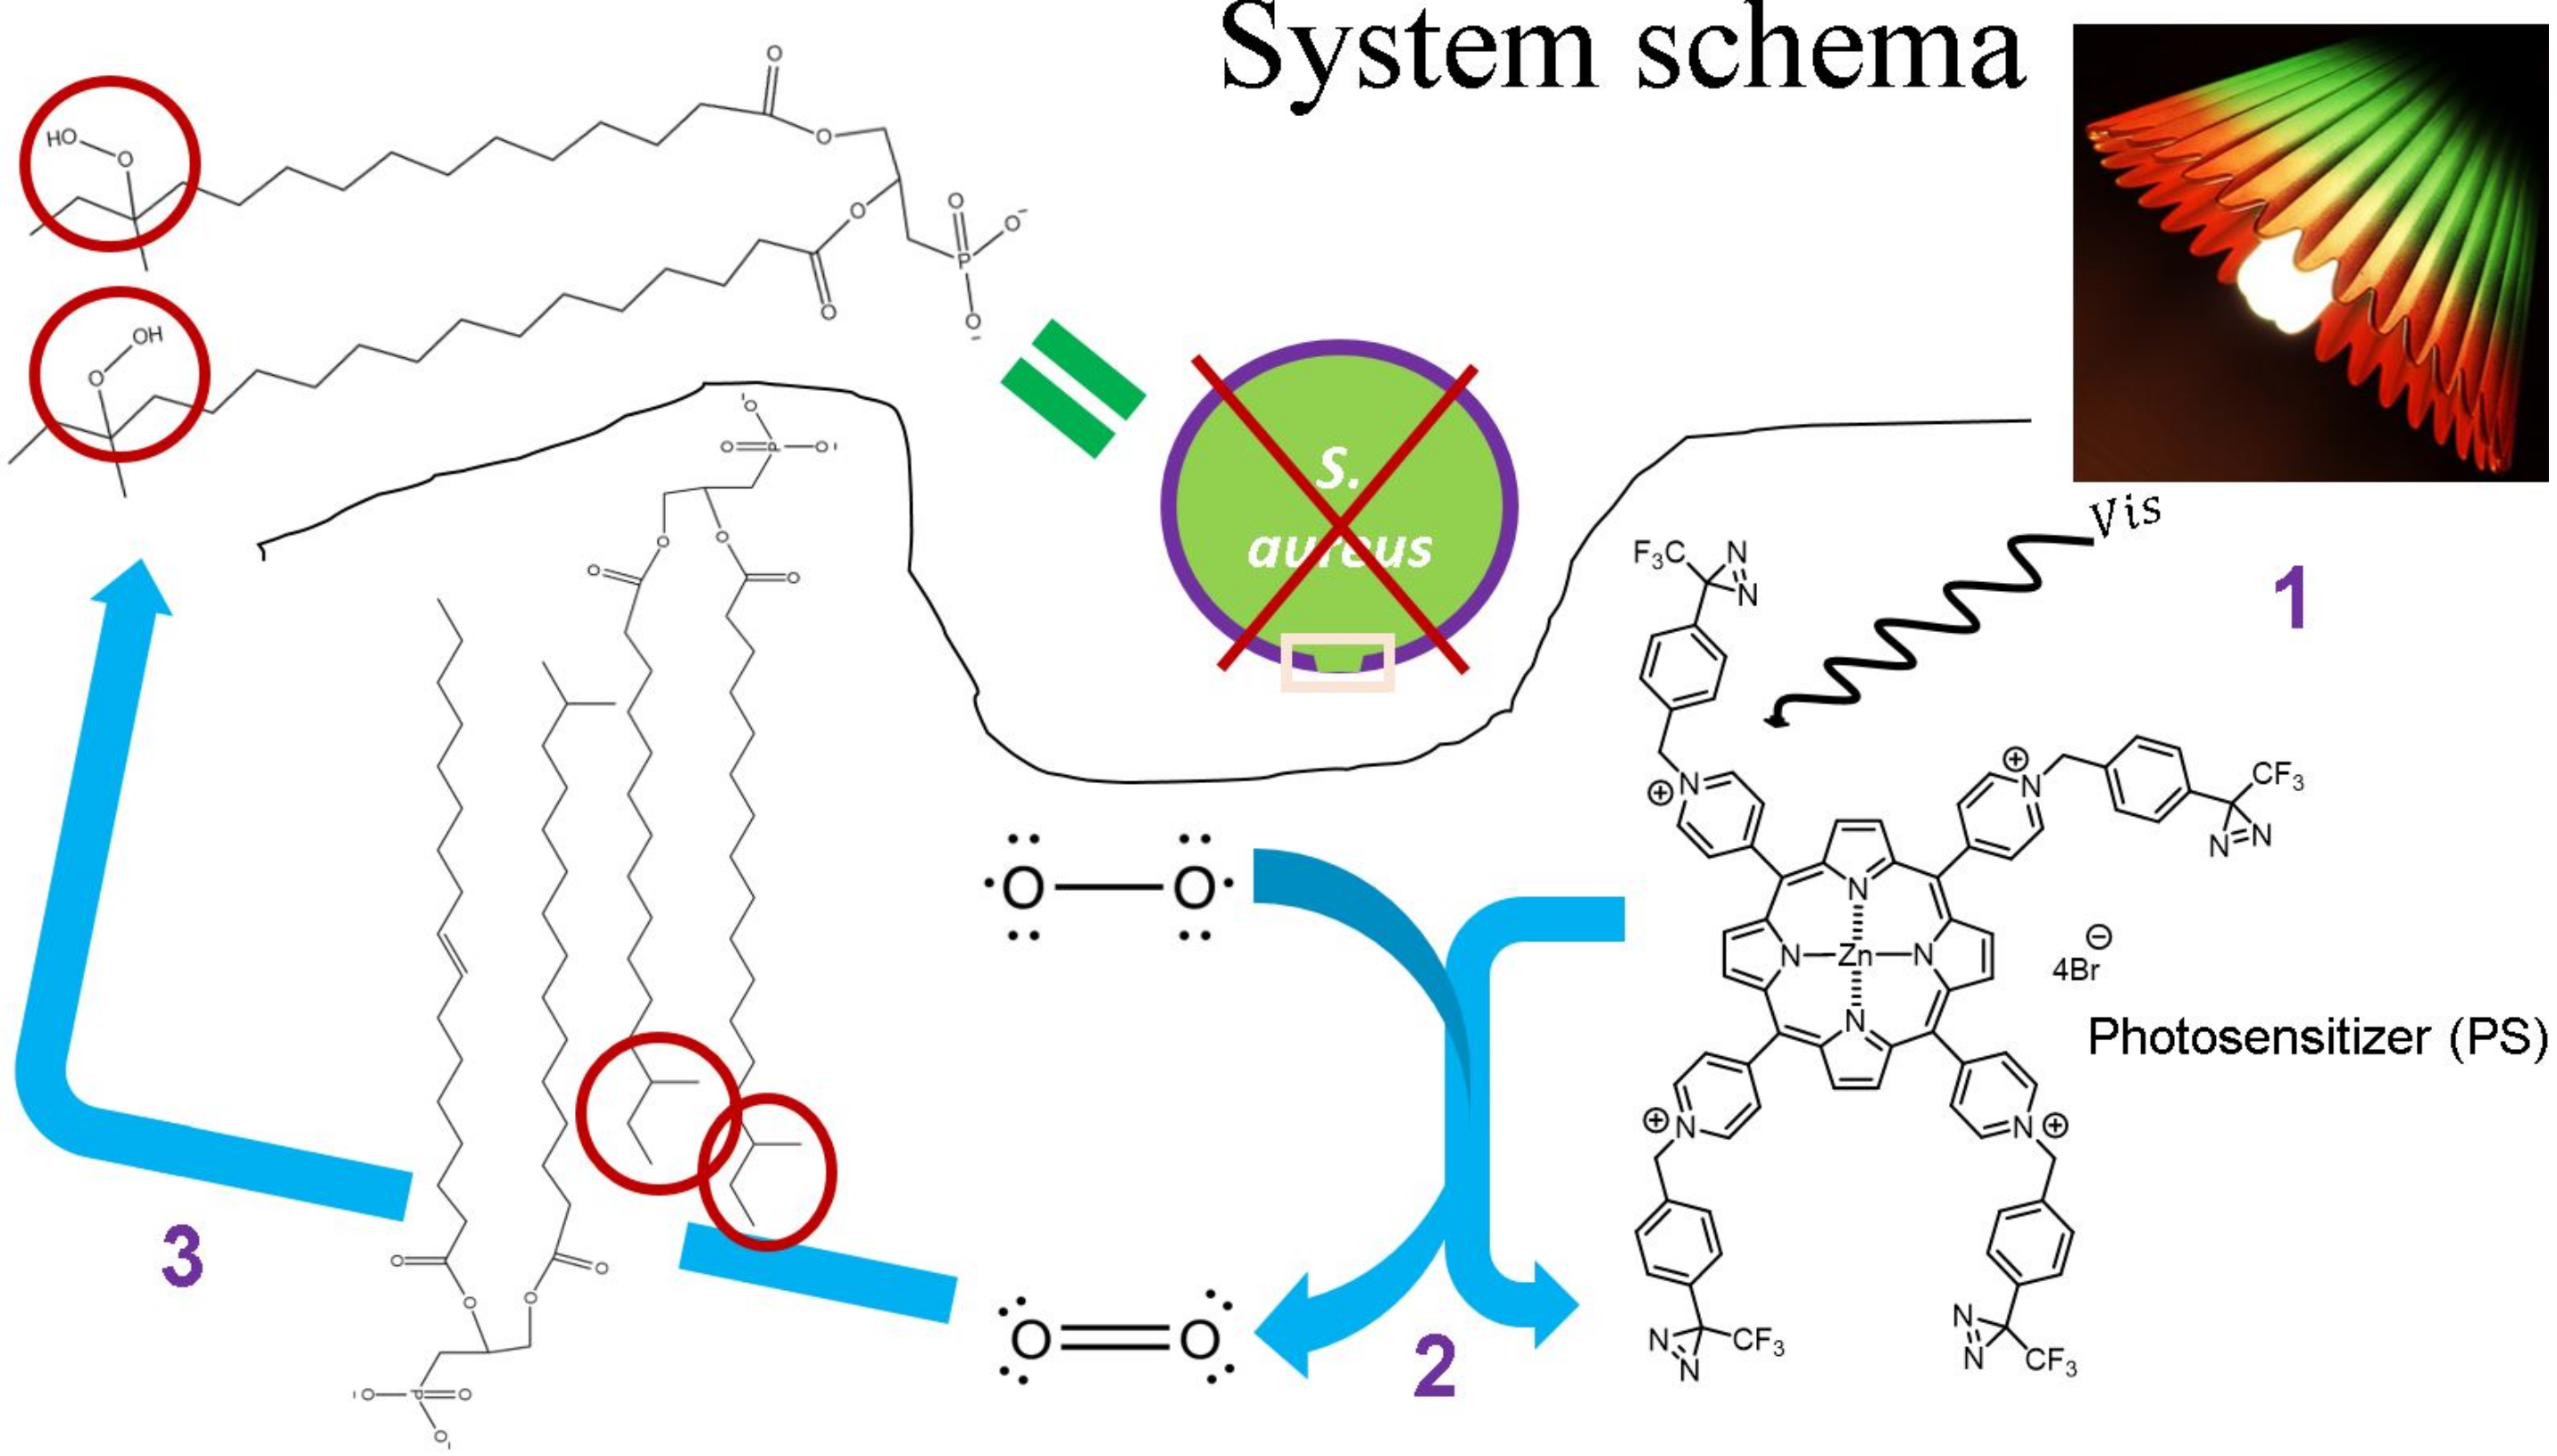
\includegraphics[width = \textwidth]{images/Introduction/PDI_workflow.png}
    \caption{
        A conceptualization of the PDI process: 1) incident light first strikes and excites a PS; 2) the excited PS catalyzes the generation of $\ce{^1O_2}$ from a ground-state oxygen; and 3) the $\ce{^3O_2}$ oxidizes a biological target to the point of cellular death.   
    }
    \label{PDI_workflow}
\end{figure}

\section{Thesis work}
All of the figures and tables in this Thesis are original. The Python modules that have been published, in the PyPI (Python Package Index) repository, at least partially for the completion of the aforementioned Thesis projects are listed in Table \ref{downloads} with their respective quantity of PyPI downloads.

\begin{table}[h]
    \centering
    \begin{tabular}{l|c|c|l}
        \textbf{Project} & \textbf{Module} & \textbf{PyPI~downloads} & \textbf{Total}\\
        \toprule
        \multirow{2}{2mm}{ROSSpy} & ROSSpy & 5,963 & \multirow{2}{2mm}{11,000}\\
         & ChemW & 4,741 & \\
         \hline
        \multirow{3}{2mm}{WCMpy} & Codons & 818 & \multirow{3}{2mm}{1,000}\\
         & BiGG\_SABIO & & \\
         & dFBApy & & \\
         \hline
        \multirow{2}{2mm}{PDIpy} & PDIpy & 561 & \multirow{2}{2mm}{5,500}\\
         & HillFit & 4,048 & \\
         \hline
         \textbf{Total} &  &  & 17,000 \\
         \bottomrule
    \end{tabular}
    \caption{
        The accumulated PyPI downloads according to PePy (\url{https://pepy.tech/}) -- per February 19th, 2022 -- for each of the modules and projects of this Thesis. 
    }
    \label{downloads}
\end{table}


\section{Future}
A few aspirations for these projects, which are detailed in Chapter 5. The most notable near-term goals include the following 4 goals. (1) Features of the modules, which are identified in their respective chapters, will be expanded to improve the utility of these tools. (2) The WCMpy suite of packages will be amalgamated into a single module that can allow experimentalists to directly simulate the biochemical effects of an anti-biofilm treatment. (3) The mature module from (2) may then be coupled with the brine predictions from ROSSpy to create a comprehensive simulation of RO desalination that embodies the reported inter-dependence of scaling and biofouling \cite{Radu2014ASystems,Radu2010ModelingPassage}. (4) Additional example cases of the PDIpy and WCMpy projects will be conducted to fortify the manuscripts for peer-review.